
In this section we provide a brief summary of the theory of
gravitational lens time delays. We have distilled much of this from the
excellent exposition of Schneider and Kochanek \citep{SKW06}, as well as
the various key papers we cite.

% Lensing, Fermat's principle and potential. Time delay surface.

Fermat's Principle of Least Time holds for the propagation of light rays
through curved spacetime. The light travel time through an isolated, thin
gravitational lens is given by
\begin{align}
    \tau(\x) &= \frac{\Ddt}{c} \cdot \Phi(\x,\y), \\
    \text{where\;\;} \Phi(\x) &= \frac{1}{2}\left(\x - \y\right)^2 - \psi(\x).
\end{align}
Here, $\x$ denotes the light source's apparent position on the sky, and
$\y$ is the position of the unlensed source. The difference between the
observable position~$\x$ and the unobservable position~$\y$ is the
scaled deflection angle~$\deflectionangle({\x})$, which is typically
$\sim1$~arcsecond in a galaxy-scale strong gravitational lens system.
$\psi(\x)$ is the scaled gravitational potential of the lensing object,
projected onto the lens plane. Both $\deflectionangle(\x)$ and $\psi(\x)$ can be
predicted given a model for the mass distribution of the lens.

Images form at the extrema of the light travel time, where $\grad
\tau(\x) = \grad \Phi(\x) = 0$ \citep{Schneider1985}. For this reason,
$\Phi(\x)$ is known as the ``Fermat potential.'' This quantity can also
be thought of as the spatially-varying refractive index of the lens. The
arrival time itself is not observable, but differences in arrival time
between multiple images are. In the above approximation, the  ``time delay'' $\Delta \tau_{\rm AB}$
between image A and
image B can be predicted via
\begin{equation}
    \Delta \tau_{\rm AB} = \frac{\Ddt}{c} \Delta \Phi_{\rm AB} \label{eq:timedelay}
\end{equation}
where $\Delta \Phi_{\rm AB}$ is the Fermat potential difference between the
two image positions.
Figure~\ref{fig:lineofsightcartoon} illustrates the origin of the
time delay between the images in a gravitational lens system. The small
magnitude of the fractional time delay (typically $\Delta\tau \sim 10$~days out of
$\Ddt/c \sim 10^{12}$ days light travel time)
is commensurate with the square of the
deflection angle (typically $|\deflectionangle|\sim1$~arcsecond, or $\sim 5\times10^{-6}$
radians).

\begin{figure*}[!t]
\centering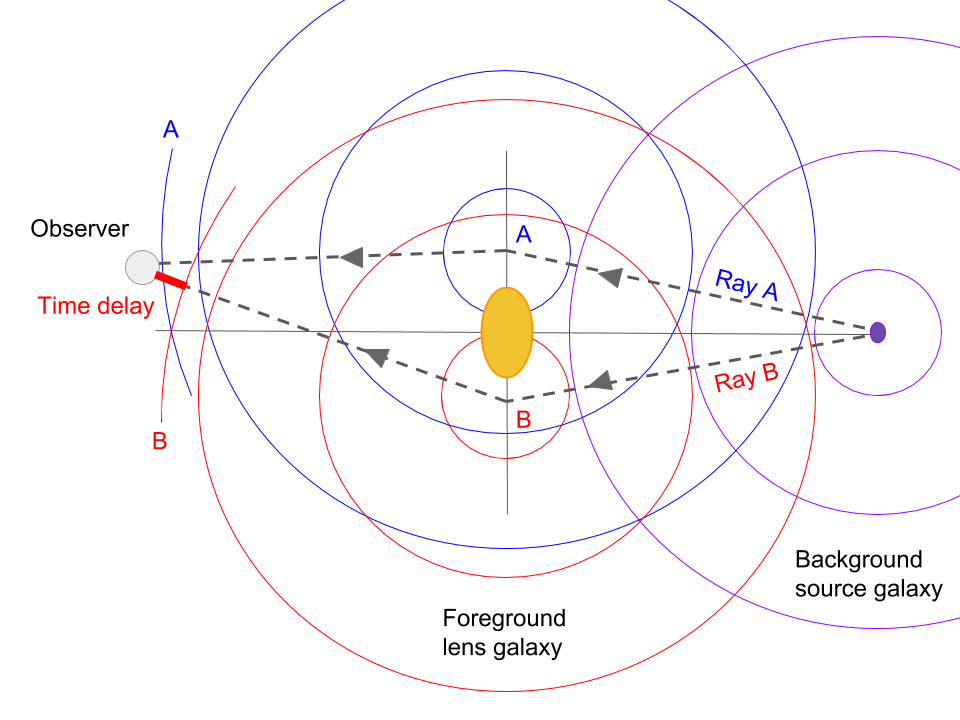
\includegraphics[width=0.96\textwidth]{figures/wavefront-schematic.png}
\caption{Schematic diagram, adapted from \citep{TreuAndEllis2015},
illustrating the origin of the gravitational time delay.}
\label{fig:timedelaycartoon}
\end{figure*}

\begin{figure*}[!ht]
\centering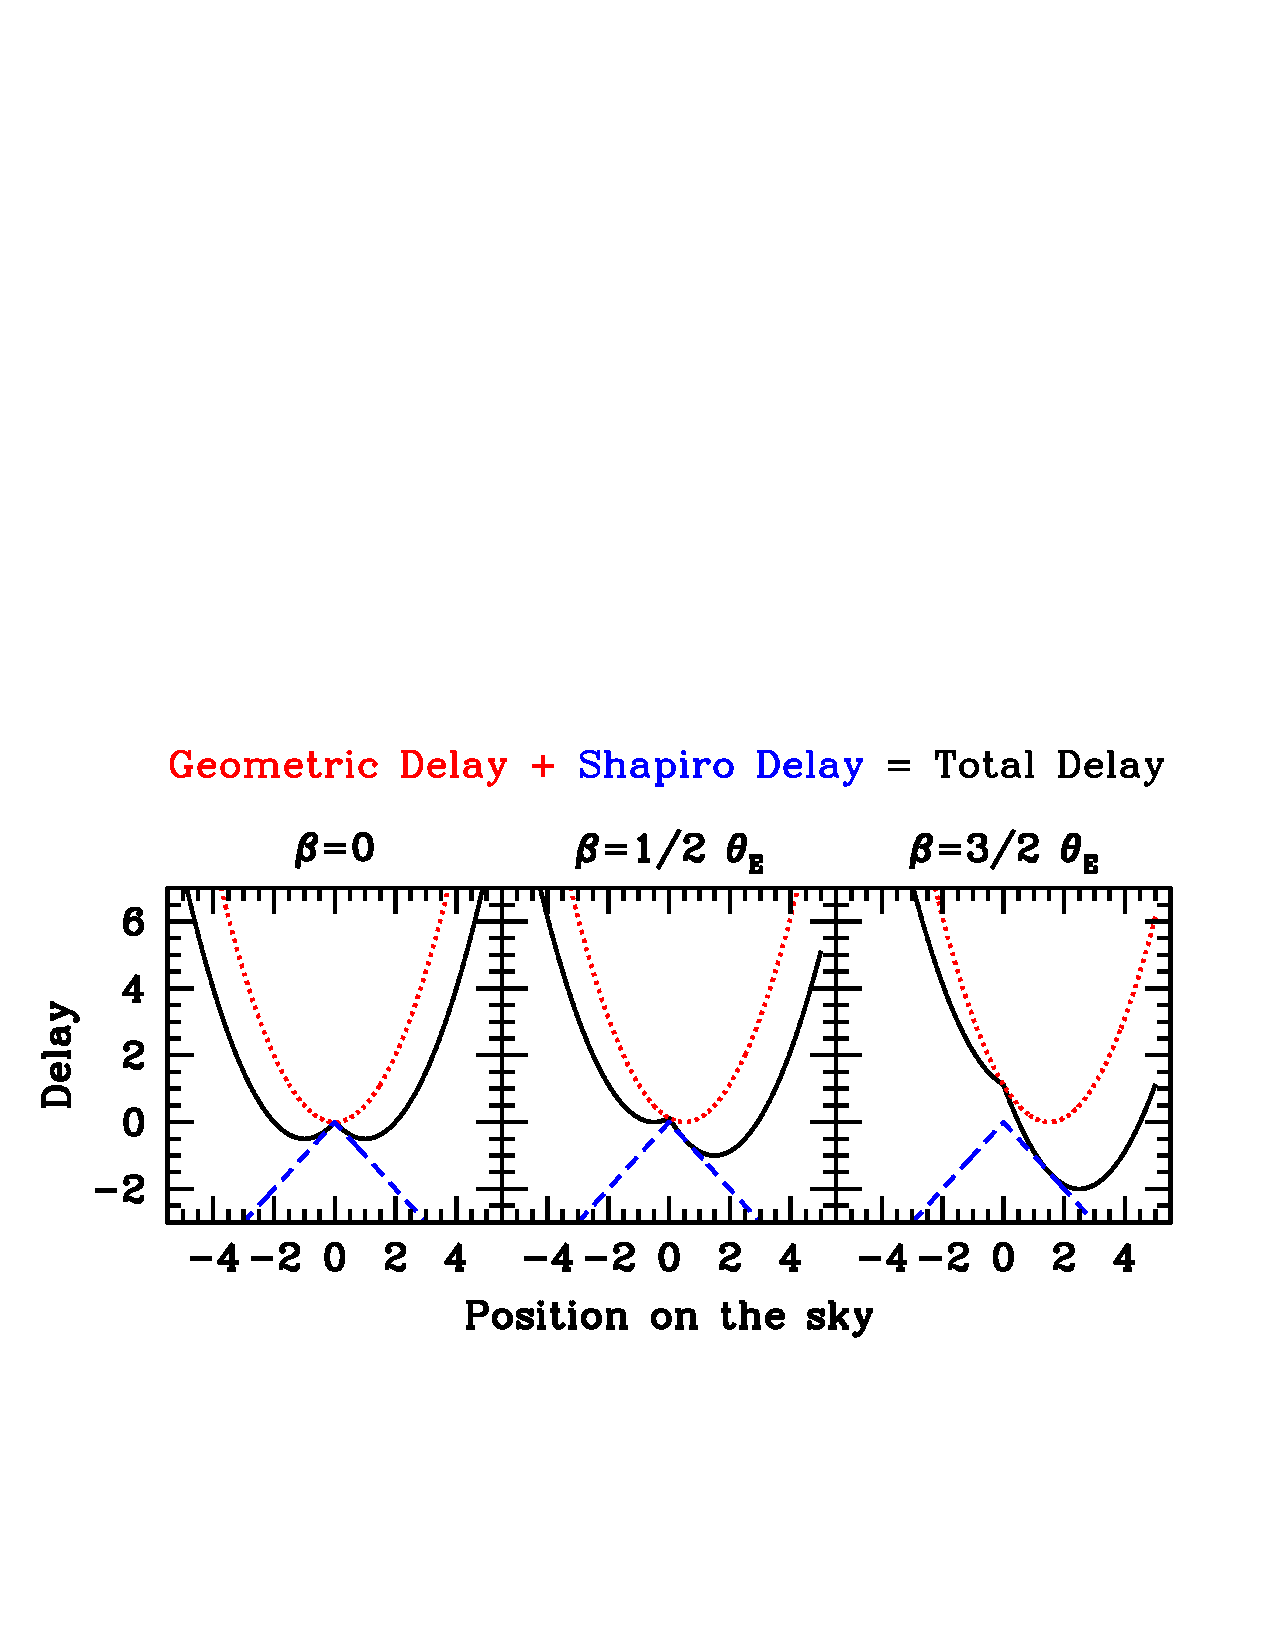
\includegraphics[width=0.96\textwidth]{figures/delays.pdf}
\caption{Geometric and general relativistic (Shapiro) contributions
to the lens time delay, from \citep{TreuAndEllis2015}. Images form
at minima and saddle points of the delay surface, shown here in
cross-section. Different source positions result in different
geometrical delays as well as shifted image positions.}
\label{fig:delays}
\end{figure*}

% Time delay distance.

We see from Equation~\ref{eq:timedelay} that given a mass
model that predicts $\Delta \Phi_{\rm AB}$, we can infer the ``time
delay distance'' $\Ddt$ from a measured time delay $\Delta \tau_{\rm AB}^{\rm obs}$.
This distance is actually a combination of angular diameter
distances:\footnote{As \citet{SKW06} point out, $\Ddt$ can be written more simply in terms
of comoving angular diameter distances, but most of the literature uses the
formula in Equation~\ref{eq:ddt}.}
\begin{equation}
    \Ddt = (1+\zd) \frac{\Dd \Ds}{\Dds}  \label{eq:ddt}
\end{equation}
These angular diameter distances can be predicted given the redshifts
of the lens and source, $\zd$ and $\zs$, and an assumed world model with
cosmological parameters~$\cospars$. The time delay distance is primarily
sensitive to the Hubble constant, since $\Ddt \propto H_0^{-1}$.

% Importance of mass distribution in lens.

Knowledge of the lens mass distribution is of vital importance to the
success of this cosmological inference: Equation~\ref{eq:timedelay}
shows  that the time delay  distance is as sensitive to uncertainty in
the predicted Fermat potential as it is the measured time delay itself.
More concentrated mass distributions with steeper density
profiles produce longer time delays leading to shorter inferred time
delay distances (and larger inferred values of $H_0$).
% Sensitivity analysis in \citep{SKW06}? Could extend to more general
% consideration of Fermat potential difference.

% Model (mass-sheet) degeneracy and its generalizations

Moreover, there is significant risk of systematic error when modeling
lens mass distributions. While image positions remain invariant under
the ``mass sheet transformation'' \citep{MSD} \citep[and its generalization, the source size transformation]{SST}, the time delays
predicted by the model can change significantly. The mass sheet transformation
and its effect on the time delay is as follows:
\begin{align}
    \kappa(\x) \rightarrow \kappa(\x)' &= \lambda + (1 - \lambda) \kappa(\x)  \label{eq:mst} \\
    \Delta \tau \rightarrow \Delta \tau' &=  (1 - \lambda) \Delta \tau.
\end{align}
This means that if we allow our model the freedom to generate both the
$\kappa(\x)$ and $\kappa(\x)'$ mass distributions, our image position
data will not favor one over the other: they will be equally likely
given the data. This model degeneracy can only be broken by additional
information. One source of information would be independent measurements
of the mass distribution: stellar kinematics is the obvious choice.
Another way to break the degeneracy is to include prior knowledge of the
lens mass distribution, from measurements of other, similar galaxies to
the lens. This type of information is typically encoded as a
simply-parametrized model, such as an elliptically-symmetric mass
distribution with power law density profile (as opposed to a free form
density map). Assuming a particular density profile partially breaks the
mass sheet degeneracy: it remains to be seen how much systematic error
in the time delay that assumption introduces.

% Importance of mass along the line sight - the universe is not Friedmann Lemaitre Robertson Walker.

The form of the mass sheet transformation given by Equation~\ref{eq:mst}
is a rescaling plus an offset. One way to achieve such a transformation
is therefore to change the overall mass of the lens,  and at the same
time add a ``mass sheet,'' a constant convergence~$\lambda$.  Both these are
possible in nature: lens galaxies come in a range of masses, and  the
combined gravitational lensing effect of all the other galaxies, groups
and filaments along  the line of sight to the source can, in the weak
lensing limit, be approximated by a constant ``external convergence''
(associate with an ``external shear'', capable of further distorting the
lensed images). This means that this additional external physical mass
component must also be taken into account when modeling the lens. It
also means that any independent information about  the physical mass of
the deflector galaxy, such as the kinematics of its  stars, can play an
important role in breaking the degeneracy in the mass model, which must
now be able to self-consistently predict the lensing effect
(image distortions and time delays) and the internal dynamics of the lens
galaxy, and take into account the weak lensing effects of structures
along the line of sight.
In Section~\ref{sec:measurement:lensmodel} we review the
recent choices and approximations that have been made when constructing
such models.


% \begin{figure*}
% % \centering\includegraphics[width=0.96\textwidth]{figures/line-of-sight-cartoon.pdf}
% \caption{Cartoon illustration of line of sight effects in time delay
% lens cosmography. Structures both within and outside the main lens
% plane provide weak deflections to the light rays, affecting both the
% image positions and time delays.} \label{fig:lineofsightcartoon}
% \end{figure*}
